\textbf{Metric.} Execution Accuracy (EX) counts a predicted query as correct when its result equals the gold query's, scored with the official Spider evaluator \cite{zhong2020semantic} (and, on BIRD, with BIRD's set comparison of results). For abstention, \emph{coverage} is the share of questions answered and \emph{accuracy on answered} the EX over those. Every number below comes from a logged run; unknown values are marked TBD.

\section{Reproduction}

Table~\ref{tab:runs} lists the runs on the Spider development set. Each step isolates a real effect: the full CodeS prompt raised the early simple-metric score from 64.8\% to 71.7\%, the authors' selection rule to 73.8\%, and the audit showed that the remaining gap was our scoring rather than the model.

\begin{table}[!t]
	\centering
	\caption{Runs on the Spider development set (1,034 questions). ``Simple'' is the early metric; only ``official'' matches the paper.}
	\label{tab:runs}
	\singlespacing
	\resizebox{\textwidth}{!}{%
	\begin{tabular}{|l|l|l|r|}
		\hline
		\textbf{Run} & \textbf{Configuration} & \textbf{Metric} & \textbf{EX} \\ \hline
		T2-001 & schema and foreign keys only; first beam & simple & 64.8\% \\ \hline
		T2-002 & full CodeS prompt; first beam & simple & 71.7\% \\ \hline
		T2-003 & + authors' candidate selection (repeated identically) & simple & 73.8\% \\ \hline
		T2-005 & audited harness & official & 77.8\% \\ \hline
		T2-006 & fresh re-run of T2-005 & official & 77.76\% (804) \\ \hline
		Paper & CodeS-1B, Table 5 of \cite{li2024codes} & official & 77.9\% \\ \hline
	\end{tabular}}
\end{table}

Scored with the paper's own evaluator, the reproduced CodeS-1B reaches \textbf{77.8\% against the reported 77.9\%}, a difference of 0.1 points, well inside the department's tolerance. Beam search is deterministic: re-runs returned identical predictions. Accuracy falls with difficulty, from 90.3\% on easy to 83.6\% on medium, 64.9\% on hard and 56.6\% on extra-hard questions; hard and extra-hard questions are a third of the set but 133 of the 230 wrong answers. Test-suite accuracy (paper: 72.2\%) is TBD.

\section{Ablation study}

Each component was disabled in turn and the full development set re-evaluated with the official evaluator (Table~\ref{tab:ablation}). Every component contributes. Without the value retriever almost as many queries still run, but with the wrong literal values, so the answers are silently wrong; candidate selection is the component that most improves executability, because it replaces a broken first beam with a working one.

\begin{table}[!t]
	\centering
	\caption{Ablation study, official evaluator (runs AB-103 to AB-106).}
	\label{tab:ablation}
	\singlespacing
	\begin{tabular}{|l|r|r|r|}
		\hline
		\textbf{Component removed} & \textbf{EX} & \textbf{Change} & \textbf{Queries that run} \\ \hline
		--- (full pipeline) & 77.8\% & --- & 97.3\% \\ \hline
		Foreign keys & 76.9\% & $-0.9$ & 95.9\% \\ \hline
		Representative column values & 76.4\% & $-1.4$ & 98.1\% \\ \hline
		Candidate selection (first beam only) & 76.0\% & $-1.8$ & 94.1\% \\ \hline
		Value retriever & 75.9\% & $-1.9$ & 97.2\% \\ \hline
	\end{tabular}
\end{table}

\section{Enhancement: confidence-aware abstention}

Table~\ref{tab:enh} compares the original and the enhanced system on the same 1,034 questions and the same predictions (run T2-006), and Table~\ref{tab:sig} gives the significance tests.

\begin{table}[!t]
	\centering
	\caption{Original against enhanced on the same 1,034 questions.}
	\label{tab:enh}
	\singlespacing
	\begin{tabular}{|l|r|r|r|}
		\hline
		\textbf{System} & \textbf{Answered} & \textbf{Accuracy on answered} & \textbf{Wrong answers} \\ \hline
		Original (reproduced CodeS-1B) & 100\% & 77.76\% & 230 \\ \hline
		Enhanced, tested setting & 90.4\% & \textbf{83.32\%} & \textbf{156} \\ \hline
		Enhanced, 3 of 4 must agree & 62.8\% & 86.13\% & 90 \\ \hline
		Enhanced, all 4 must agree & 39.8\% & 88.35\% & 48 \\ \hline
	\end{tabular}
\end{table}

\begin{table}[!t]
	\centering
	\caption{Significance over 10 calibration/test splits and a 5,000-sample bootstrap over questions.}
	\label{tab:sig}
	\singlespacing
	\resizebox{\textwidth}{!}{%
	\begin{tabular}{|l|l|l|l|l|}
		\hline
		\textbf{Signal} & \textbf{Mean gain} & \textbf{Paired t-test (df 9)} & \textbf{Wilcoxon} & \textbf{Bootstrap 95\% CI} \\ \hline
		Execution agreement & $+5.46$ pts & $t = 24.44$, $p = 7.7 \times 10^{-10}$ & $W = 55$, $p = 9.8 \times 10^{-4}$ & $[+4.51, +6.71]$ \\ \hline
		Beam probability (comparison) & $+3.08$ pts & $t = 10.81$, $p = 9.3 \times 10^{-7}$ & $W = 55$, $p = 9.8 \times 10^{-4}$ & $[+1.97, +3.94]$ \\ \hline
	\end{tabular}}
\end{table}

H0 is rejected: all 10 splits show a gain, and no bootstrap resample shows a gain of zero or less. At the tested setting the system declines 99 questions, 74 of which it would have answered wrongly: wrong answers fall by 32\% at the cost of withholding 3.1\% of the correct ones. The signal is calibrated --- accuracy rises with agreement, from 0\% when the selected query does not run (28 questions) to 56.8\% at 1 of 4, 75.6\% at 2, 82.3\% at 3 and 88.3\% at 4 of 4 --- and Figure~\ref{fig:coverage} shows the whole accuracy--coverage curve.

\begin{figure}[!t]
	\centering
	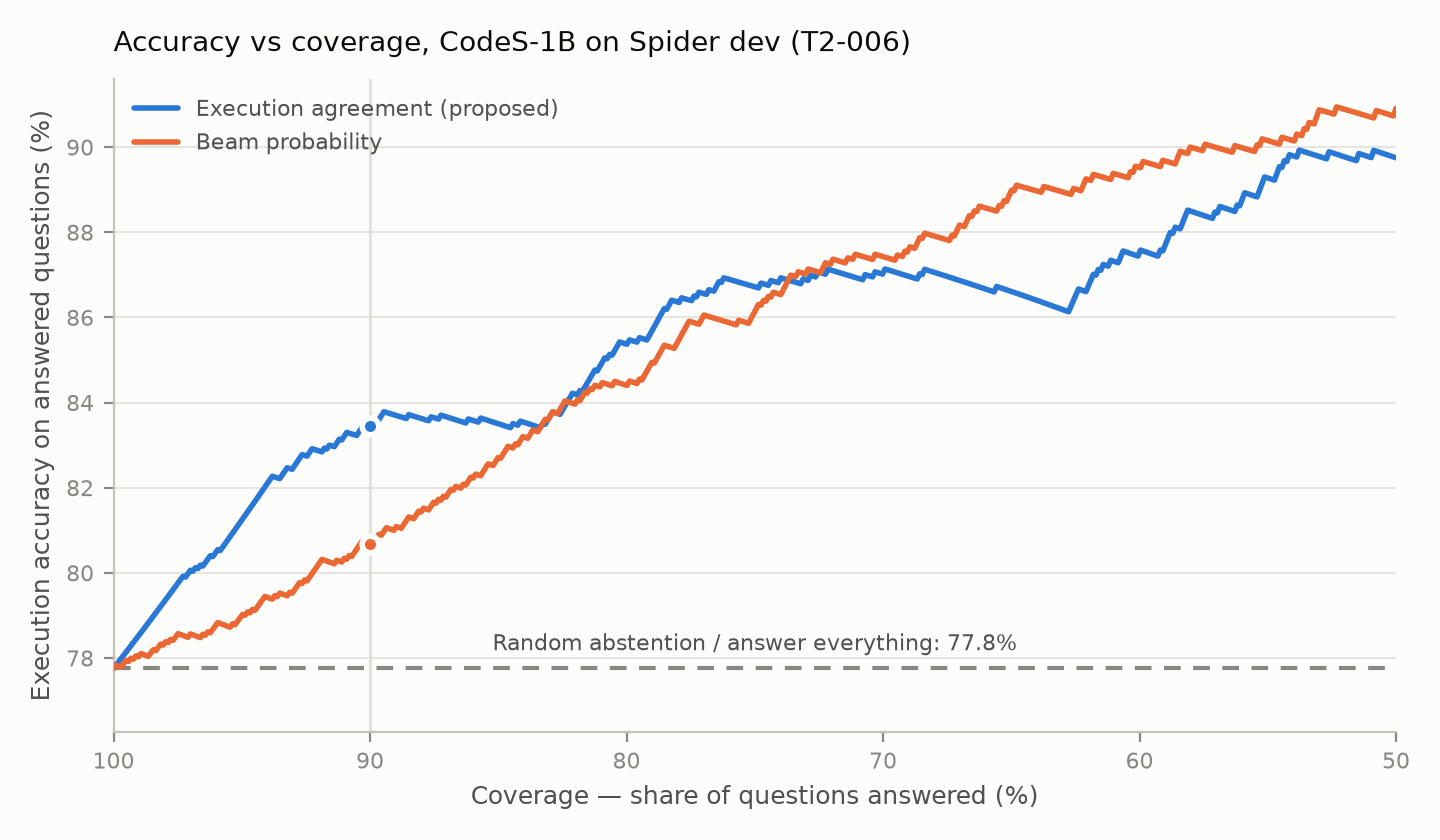
\includegraphics[width=0.75\linewidth]{images/figures/accuracy_coverage_T2-006.png}
	\caption{Accuracy on answered questions against coverage; the dashed line is the original system (and random abstention).}
	\label{fig:coverage}
\end{figure}

\textbf{What the enhancement does not do.} Plain Execution Accuracy stays at 77.8\%: the gain is in the answers the system gives, not in answering more questions correctly. Using agreement to \emph{choose} the answer (majority vote) instead of only to decide whether to trust it lowers EX to 75.73\%, although a correct query is among the four candidates for 83.08\% of questions --- room for a learned reranker.

\section{Self-correction (application feature)}

Keeping the T2-006 candidates fixed, every failed candidate (377 queries in 211 questions) was sent back to CodeS-1B once with its database error (run RP-001). Only 61 repaired queries ran and one answer became correct: EX moved from 77.76\% to 77.85\%, and the tested abstention setting from 83.32\% to 83.23\% at 90.5\% coverage. CodeS was fine-tuned on question--SQL pairs and never learned to use error feedback, which confirms the choice of enhancement. The application's later repairs (stored-value hints for empty answers, joins for misplaced columns) are not measured.

\section{Benchmark-to-reality gap}

The evaluated CodeS-1B pipeline was run unchanged, with the abstention threshold calibrated on Spider. On Spider-Realistic every question is paired with its original Spider wording and both were run on the same machine (run RL-001, Apple M4), so the difference measures the wording alone (Table~\ref{tab:real}).

\begin{table}[!t]
	\centering
	\caption{The same 508 questions in their original and their realistic wording (run RL-001).}
	\label{tab:real}
	\singlespacing
	\begin{tabular}{|l|r|r|}
		\hline
		 & \textbf{Original wording} & \textbf{Realistic wording} \\ \hline
		Execution Accuracy, answering everything & 72.8\% (370) & 69.5\% (353) \\ \hline
		Paper, SFT CodeS-1B (Table 7 of \cite{li2024codes}) & --- & 70.9\% \\ \hline
		Balanced setting: questions answered & 88.6\% & 86.2\% \\ \hline
		Balanced setting: accuracy on answered & 79.3\% & 76.7\% \\ \hline
		Wrong answers: answering everything $\rightarrow$ balanced & 138 $\rightarrow$ 93 & 155 $\rightarrow$ 102 \\ \hline
	\end{tabular}
\end{table}

\textbf{A second reproduction point.} On Spider-Realistic we obtain 69.5\% against the paper's 70.9\% for SFT CodeS-1B, a difference of 1.4 points, inside the tolerance. As a hardware check, on the 508 original-wording questions this run chose the same query as the Colab run T2-006 for 485 questions, with 72.8\% against 73.2\% accuracy.

\textbf{The wording gap.} Removing the column names costs 3.3 points (bootstrap 95\% CI $[0.8, 5.9]$): 31 questions are right only in the original wording and 14 only in the realistic one (exact McNemar $p = 0.016$), so the drop is real but small. Abstention keeps working on the realistic wording without recalibration: accuracy still rises with agreement (47.1\% at 1 of 4, 86.9\% at 4 of 4), and the balanced setting removes a third of the wrong answers (155 to 102) at 86.2\% coverage.

\textbf{Real-world databases.} The BIRD Mini-Dev evaluation (run BD-001) was in progress when this report was printed; its result is TBD.
